\section{Resultados}

El sintonizador de parámetros obtuvo los mejores parámetros para las dos ins-tancias analizadas, los cuales se muestran en la Tabla \ref{tab:mejoresparam}.

\begin{table}[!htb]
\begin{center}
\begin{tabular}{|l|r|r|r|r|r|}
\hline
Instancia & \pmejores & \pclones & \preemplazo & \popsize & \clonsize \\
\hline
\hline
Mandl & 1.00 & 0.25 & 0.30 & 150 & 200 \\
\hline
Mumford0 & 0.25 & 0.25 & 0.30 & 150 & 150 \\
\hline
\end{tabular}
\end{center}
\caption{Valores entregados por el sintonizador para cada instancia.}
\label{tab:mejoresparam}
\end{table}

De acuerdo a estos resultados, se puede apreciar que el parámetro \pmejores{} se mantuvo en el valor por defecto para Mandl, pero disminuyó al mínimo posible en Mumford0. Probablemente, esto se debe a que la red de Mumford0 es más grande y se tiene mejor esperanza de mejorar las soluciones si se toma una fracción de las mejores soluciones para pasar al proceso de mutación.

El mejor valor para el parámetro \pclones{} fue asignado al mínimo posible en ambas instancias, lo que indica que se toma una fracción pequeña de valores para almacenar en el conjunto de memoria, lo que tiene una ventaja computacional al evitar almacenar soluciones que podrían ser eliminadas posteriormente. 

El parámetro \preemplazo{} se mantuvo en el valor por defecto sugerido en ambas instancias y probablemente es el mejor valor para un \textit{trade-off} entre exploración y explotación en una vecindad de soluciones candidatas.

Los tamaños de población, reflejados en los parámetros \popsize{} y \clonsize{} aumentaron con respecto a los valores por defecto. Al comparar las cantidades de ambas poblaciones, se cumple que el tamaño de la población de clones siempre es mayor o igual al tamaño de la población de cada generación.

\begin{figure}[!htb]
\centering
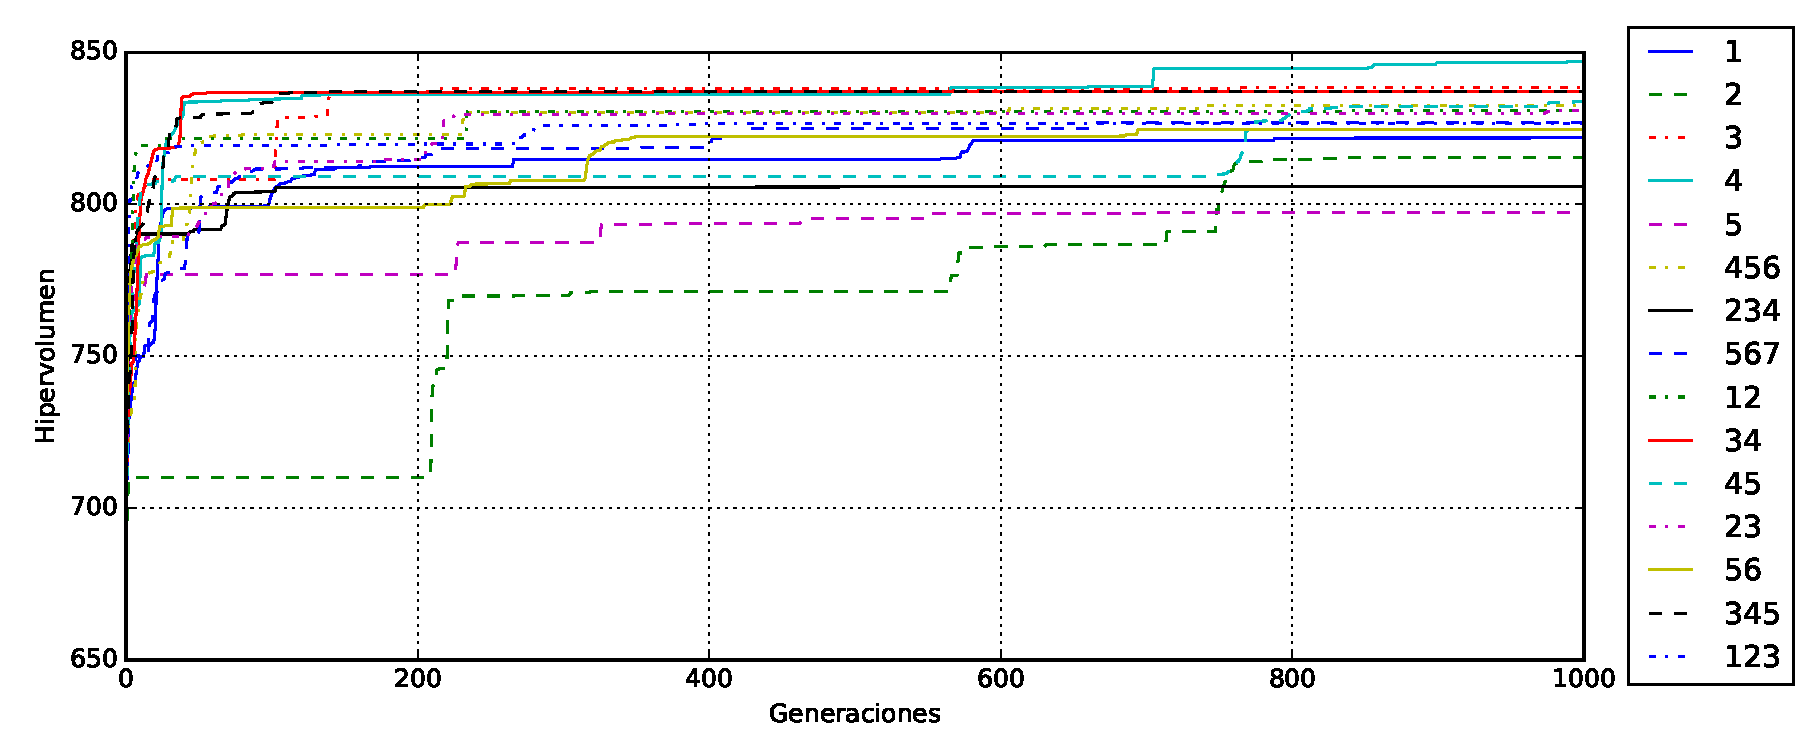
\includegraphics[width=\textwidth]{img/hyp_Mandl}
\caption{Hipervolumen obtenido en 15 semillas distintas con la instancia Mandl con sintonización de parámetros.}
\label{fig:hyp_mandl}
\end{figure}

\begin{figure}[!htb]
\centering
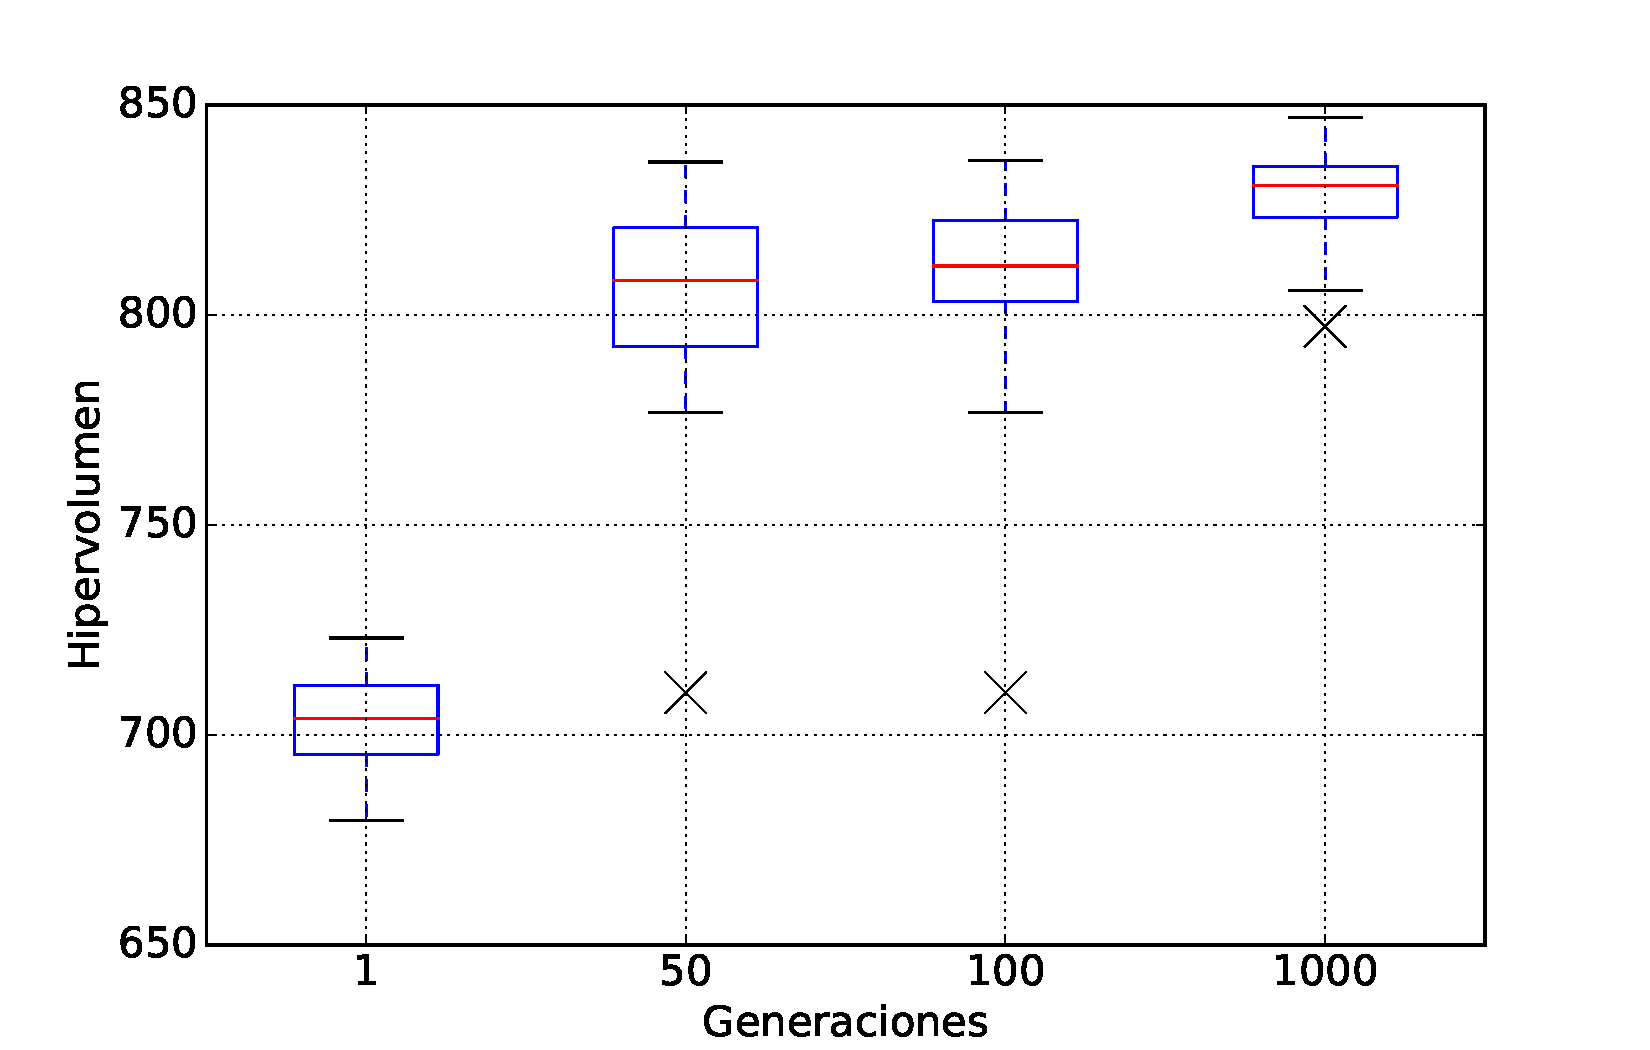
\includegraphics[width=\textwidth]{img/hyp_Mandl_bp}
\caption{Box plot del hipervolumen obtenido en distintas generaciones del algoritmo inmune para la instancia Mandl con sintonización de parámetros.}
\label{fig:hyp_mandl_bp}
\end{figure}

Al realizar experimentos para la instancia de Mandl con los mejores valores de los parámetros con 15 semillas distintas, se puede observar la variación de hipervolumen para todas ellas en la Figura \ref{fig:hyp_mandl}. Se aprecia que el comportamiento de la gráfica es el esperado para un algoritmo que va mejorando sus soluciones en cada generación. Se observa que en todos los casos hay periodos de estancamiento en las soluciones obtenidas, pero en ocasiones se produce una mejora súbita para pasar nuevamente a otro periodo de estancamiento. En general, a partir de la generación 200 no se observa una gran mejora en las soluciones obtenidas, ya que el hipervolumen se mantiene en niveles estables para cada caso. La Figura \ref{fig:hyp_mandl_bp} muestra la distibución de los valores del hipervolumen obtenidos con las 15 semillas en las generaciones 1, 50, 100 y 1000 del algoritmo para la instancia Mandl, utilizando los mejores valores de los parámetros para esta instancia. Se observa que a medida que aumentan las generaciones del algoritmo la mayoría de los valores se acerca a un valor de hipervolumen comprendido entre 800 y 850. Se puede decir entonces, que el algoritmo inmune propuesto no es afectado en gran medida por la aleatoridad introducida al utilizar distintas semillas en esta instancia.

A continuación, los frentes de Pareto resultantes de 4 semillas se pueden apreciar en las Figuras \ref{fig:paretoMandl1} y \ref{fig:paretoMandl2}. Además, información adicional de apoyo referente a estos frentes se encuentra en la Tabla \ref{tab:dataFrenteMandl}. En los casos mostrados, se observa que los frentes de Pareto se acercan a los mínimos de ambas funciones a medida que aumenta el número de generaciones. Adicionalmente, se puede ver la aparición de nuevas soluciones que no estaban definidas con anterioridad. El algoritmo propuesto es capaz de encontrar nuevas soluciones dentro de un vecindario de soluciones similares, producto de los operadores de mutación aplicados, los cual queda en evidencia con el aumento de soluciones del frente al aumentar el número de generaciones. Por otra parte, se obtienen mejoras en las soluciones ya encontradas, al visualizar el avance del frente de Pareto hacia el sector inferior izquierdo que tiene los mínimos de las dos funciones objetivo. Otro aspecto a notar en estas gráficas es la forma en que los frentes se van acercando al sector inferior izquierdo. Se observa claramente que el algoritmo propuesto obtiene muchas soluciones que son buenas para los operadores y pocas soluciones que son buenas para los pasajeros. 

\begin{figure}[p]
\centering
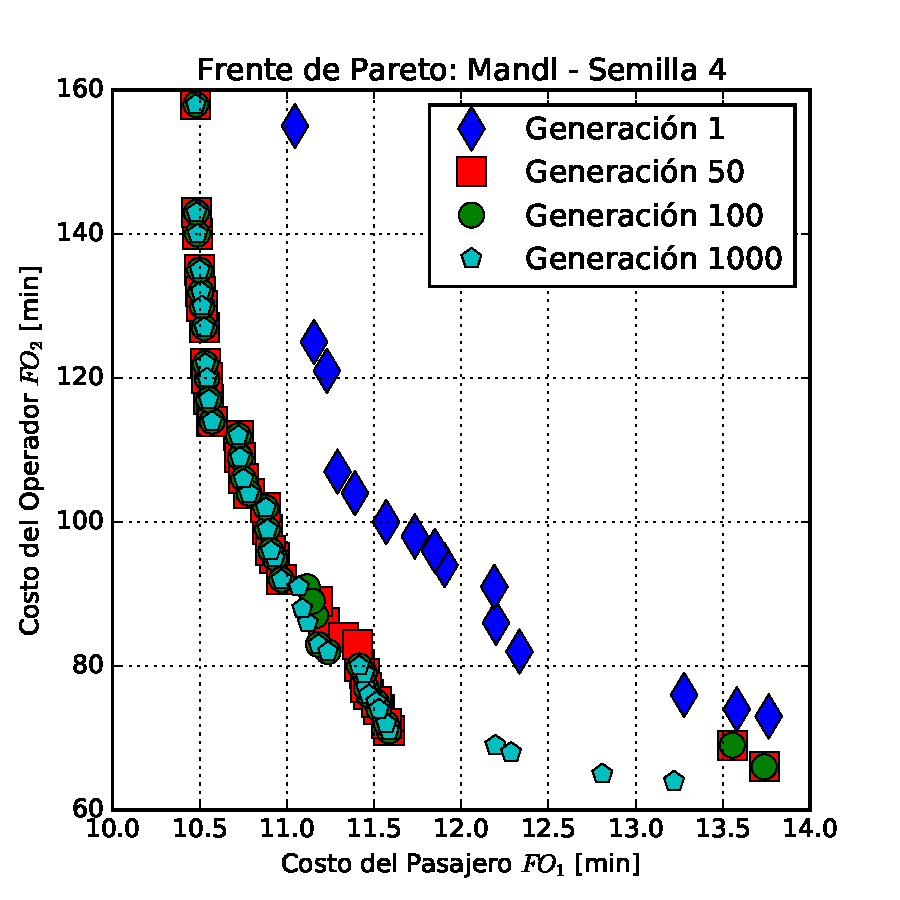
\includegraphics[width=0.79\textwidth]{img/frente_Mandl_s4}
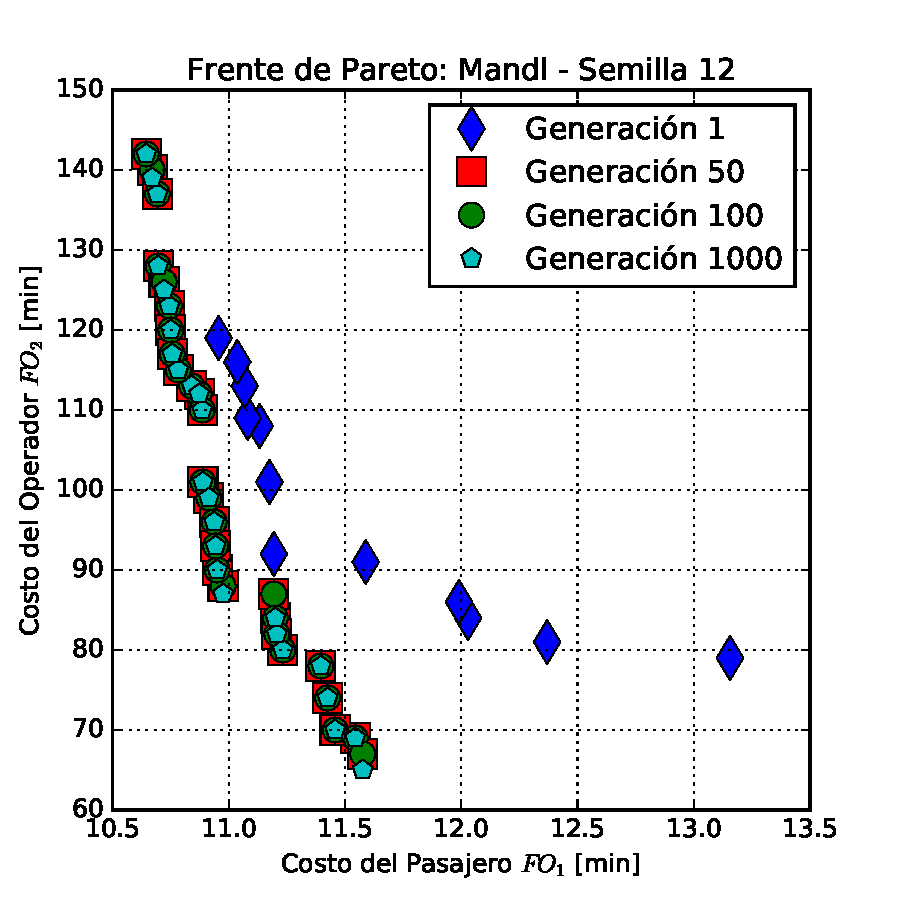
\includegraphics[width=0.79\textwidth]{img/frente_Mandl_s12}
\caption{Frente de Pareto para Mandl con semillas 4 y 12.}
\label{fig:paretoMandl1}
\end{figure}

\begin{figure}[p]
\centering
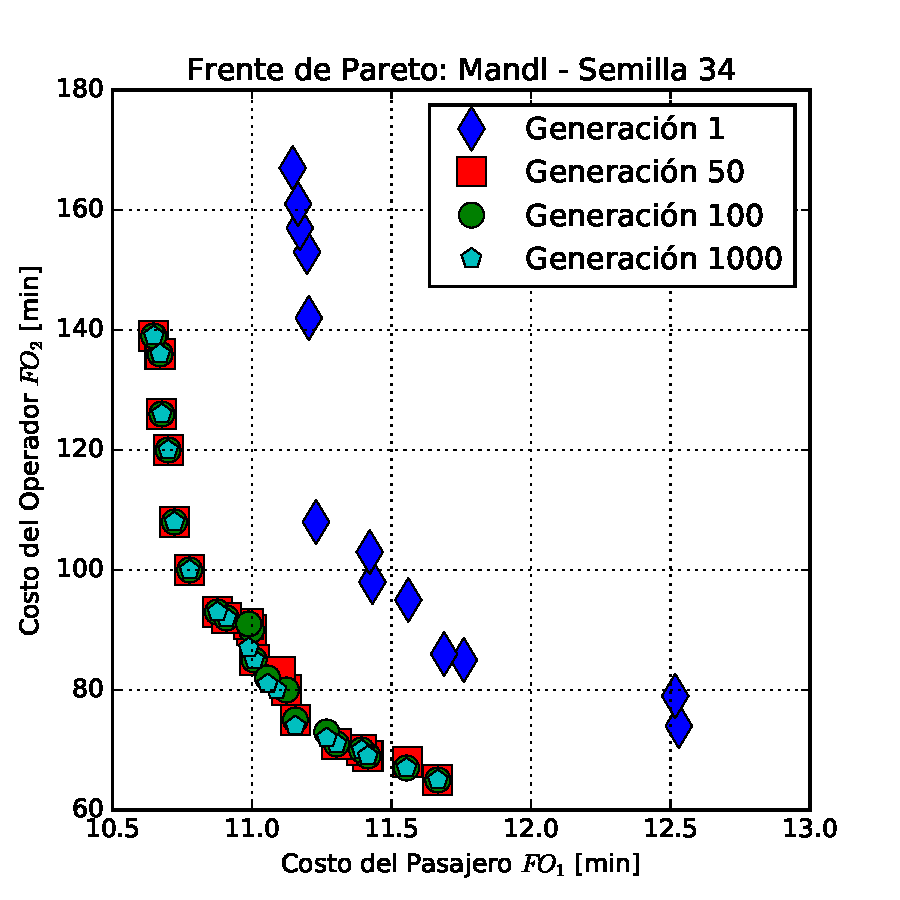
\includegraphics[width=0.79\textwidth]{img/frente_Mandl_s34}
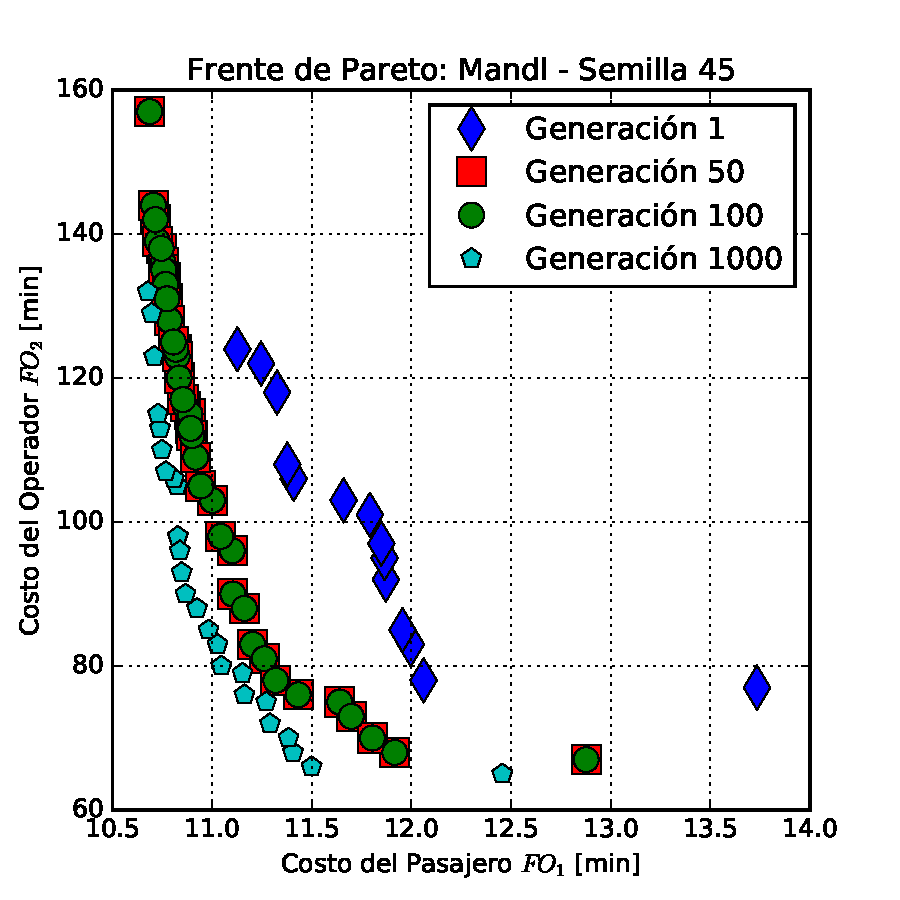
\includegraphics[width=0.79\textwidth]{img/frente_Mandl_s45}
\caption{Frente de Pareto para Mandl con semillas 34 y 45.}
\label{fig:paretoMandl2}
\end{figure}

\begin{table}[!htb]
\centering
\begin{tabular}{|r|r|r|r|r|r|}
\hline
Semilla & Generación & Sol. Únicas & Sol. Totales & Hipervolumen & Tiempo [s]\\ 
\hline \hline
4 & 1 & \textbf{15} & \textbf{15} & 702.207 & 26 \\ \hline
45 & 1 & 14 & 14 & 692.819 & 25 \\ \hline
12 & 1 & 12 & 12 & \textbf{714.867} & \textbf{22} \\ \hline
34 & 1 & 13 & 13 & 704.389 & \textbf{22} \\ \hline \hline
4 & 50 & 34 & 34 & 833.746 & 334 \\ \hline
45 & 50 & \textbf{36} & \textbf{36} & 809.110 & 344 \\ \hline
12 & 50 & 27 & 27 & 821.737 & 347 \\ \hline
34 & 50 & 19 & 19 & \textbf{836.426} & \textbf{325} \\ \hline\hline
4 & 100 & 35 & 65 & 834.683 & 645 \\ \hline
45 & 100 & \textbf{36} & \textbf{70} & 809.110 & 663 \\ \hline
12 & 100 & 27 & 27 & 821.737 & 683 \\ \hline
34 & 100 & 20 & 37 & \textbf{836.769} & \textbf{634} \\ \hline \hline
4 & 1000 & \textbf{37} & \textbf{335} & 847.025 & 6770 \\ \hline
45 & 1000 & 25 & 83 & 833.812 & 6533 \\ \hline
12 & 1000 & 26 & 153 & 830.848 & 6675 \\ \hline
34 & 1000 & 19 & 180 & \textbf{837.087} & \textbf{6357} \\ \hline
\end{tabular}
\caption{Cantidad de soluciones únicas/totales, hipervolumen y tiempo de cómputo en el frente de Pareto para 4 semillas de la instancia Mandl.}
\label{tab:dataFrenteMandl}
\vspace{0.5cm}

\end{table}

Por medio de la información de la Tabla \ref{tab:dataFrenteMandl} se destaca para este algoritmo en específico la aparición de muchas soluciones idénticas en los frentes de Pareto. Se puede observar, a modo general que desde la generación 50 y la generación 100 la soluciones totales son el doble de las soluciones únicas. En la generación 1000, las soluciones únicas representa entre un 10\% y un 30\% de las soluciones totales. En esta instancia se mantiene la tendencia de que la semilla que genera más soluciones únicas es la que tiene más soluciones totales. No existe una correlación entre un mayor hipervolumen con más soluciones únicas/totales en el frente. Finalmente, el tiempo para una instancia fue medido desde el inicio del algoritmo hasta la finalización de una generación. Tiempos menores en etapas prematuras del algoritmo suelen derivar en un tiempo total de cómputo menor para el algoritmo completo. Notar que al término de la generación 1 han transcurrido cerca de 20 segundos desde el inicio del algoritmo, donde este tiempo está destinado a la generación del conjunto inicial de soluciones factibles para iniciar el algoritmo.

En el caso de la instancia Mumford0, se realizó el mismo procedimiento, utilizando 15 semillas distintas con 1000 generaciones y los mejores valores  para los parámetros. La Figura \ref{fig:hyp_mumford0} muestra la evolución del hipervolumen para todas las semillas utilizadas y la Figura \ref{fig:hyp_mumford0_bp} muestra la distribución de los valores de hipervolumen para las semillas en las generaciones 1, 50, 100 y 1000 del algoritmo. En la Figura \ref{fig:hyp_mumford0} se observa que el hipervolumen aumenta su valor en todas las semillas utilizadas, notando estancamientos prolongados en este valor desde las 200 generaciones aproximadamente. En el \textit{box plot} de la Figura \ref{fig:hyp_mumford0_bp} se puede notar la aparición de \textit{outliers}. Sin embargo, para todas las semillas se observa el mismo comportamiento creciente, visto anteriormente. A modo general, el algoritmo no se ve afectado por la aleatoridad de una semilla determinada y tiende a obtener un valor de hipervolumen acotado.

\begin{figure}[!htb]
\centering
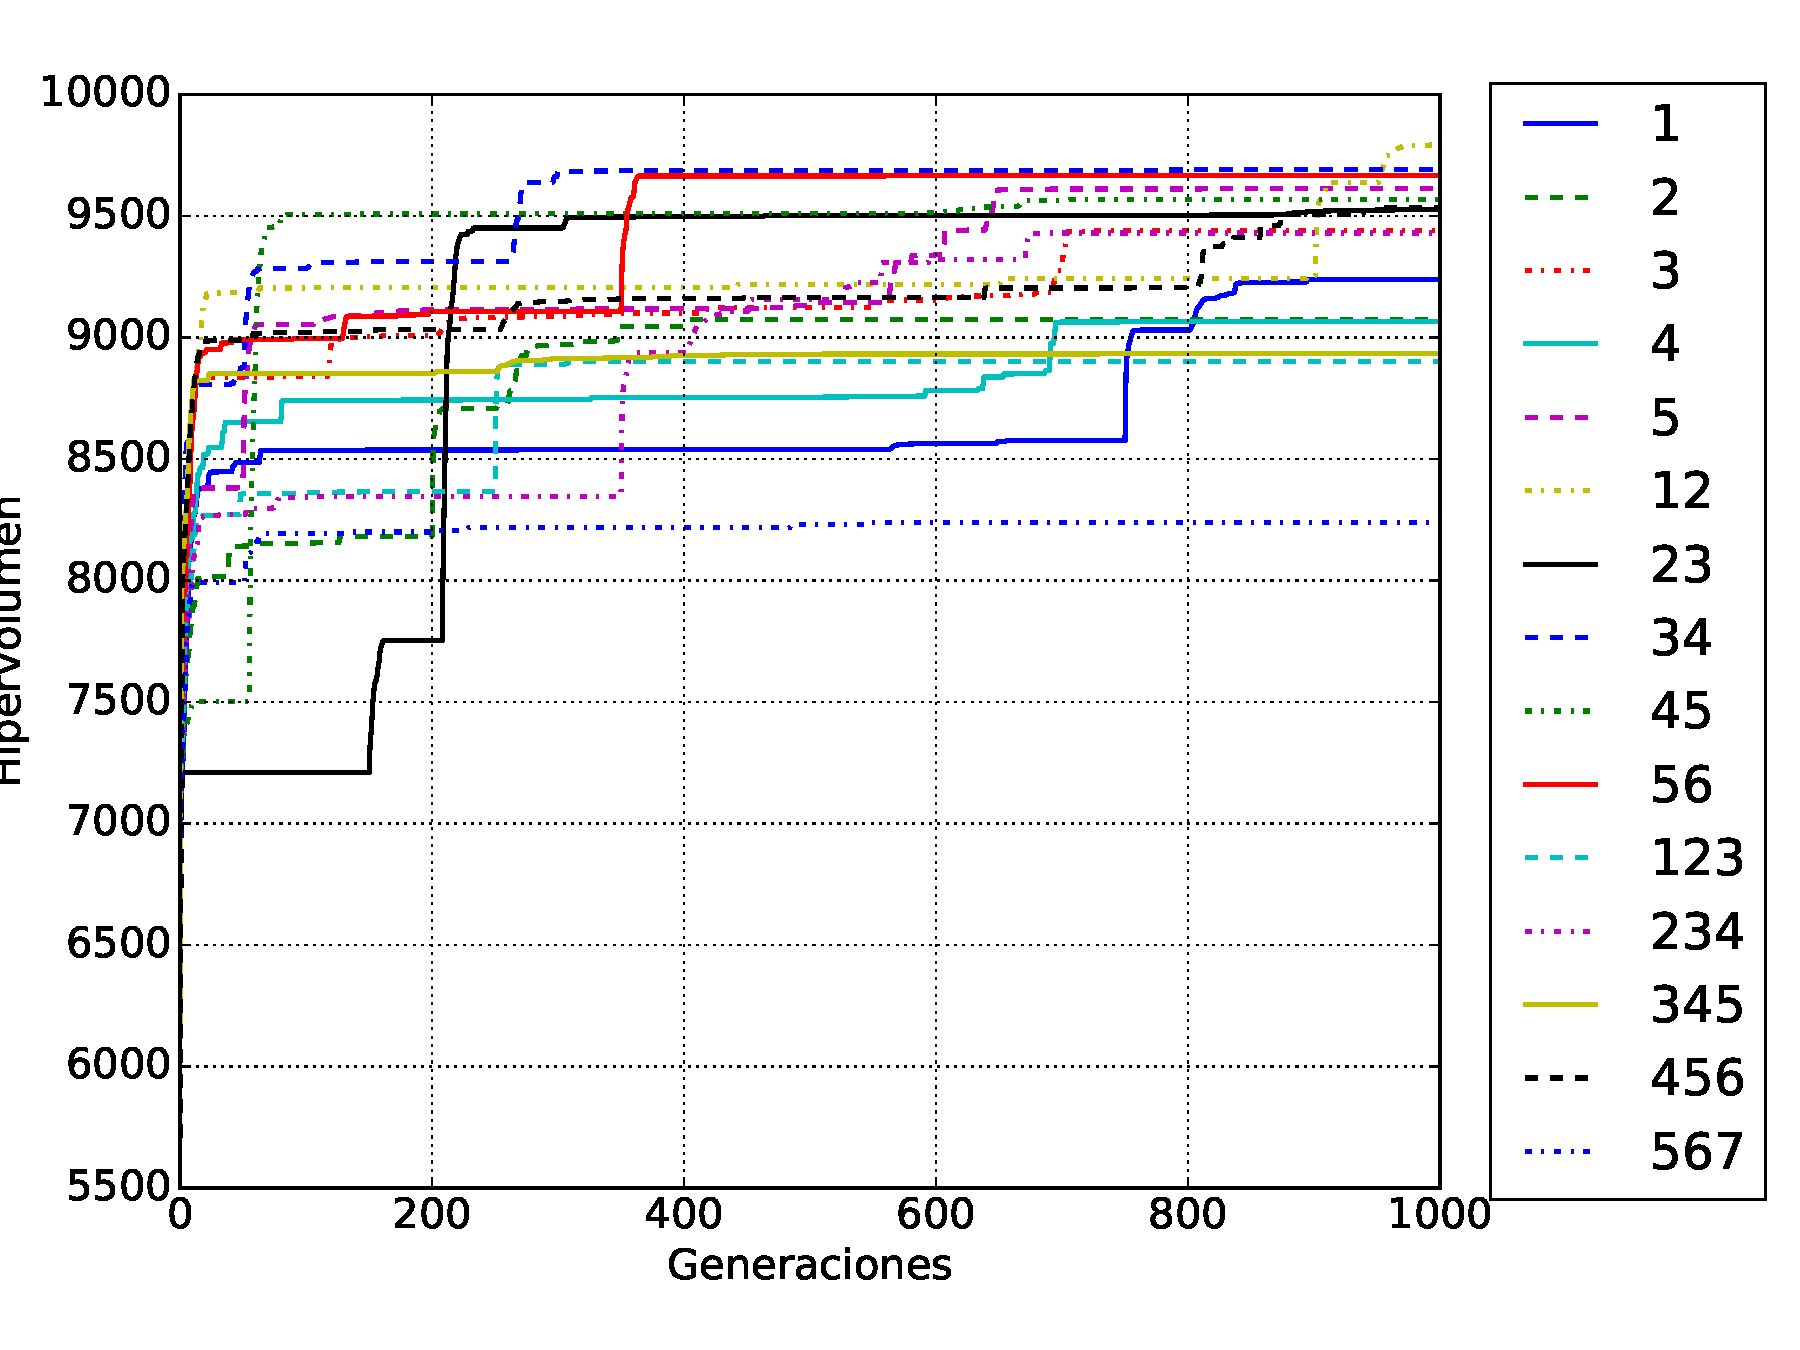
\includegraphics[width=\textwidth]{img/hyp_Mumford0}
\caption{Hipervolumen obtenido en 15 semillas distintas con la instancia Mumford0 con sintonización de parámetros.}
\label{fig:hyp_mumford0}
\end{figure}

\begin{figure}[!htb]
\centering
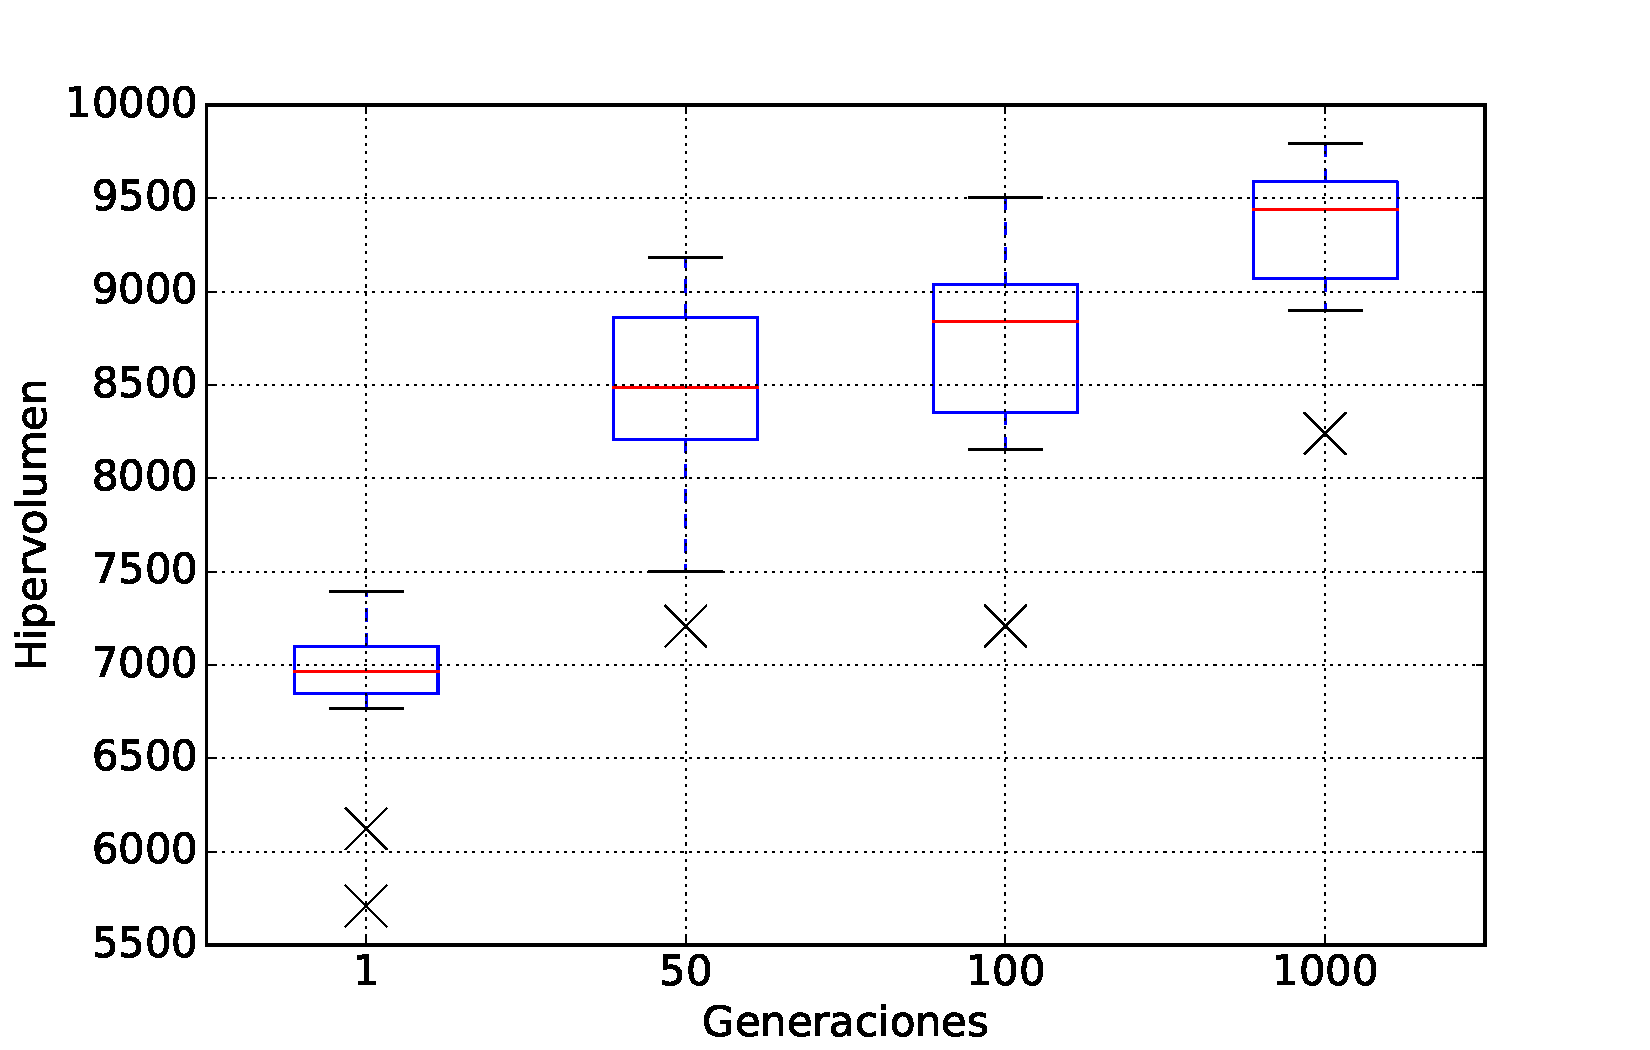
\includegraphics[width=\textwidth]{img/hyp_Mumford0_bp}
\caption{Box plot del hipervolumen obtenido en distintas generaciones del algoritmo inmune para la instancia Mumford0 con sintonización de parámetros.}
\label{fig:hyp_mumford0_bp}
\end{figure}

\begin{figure}[p]
\centering
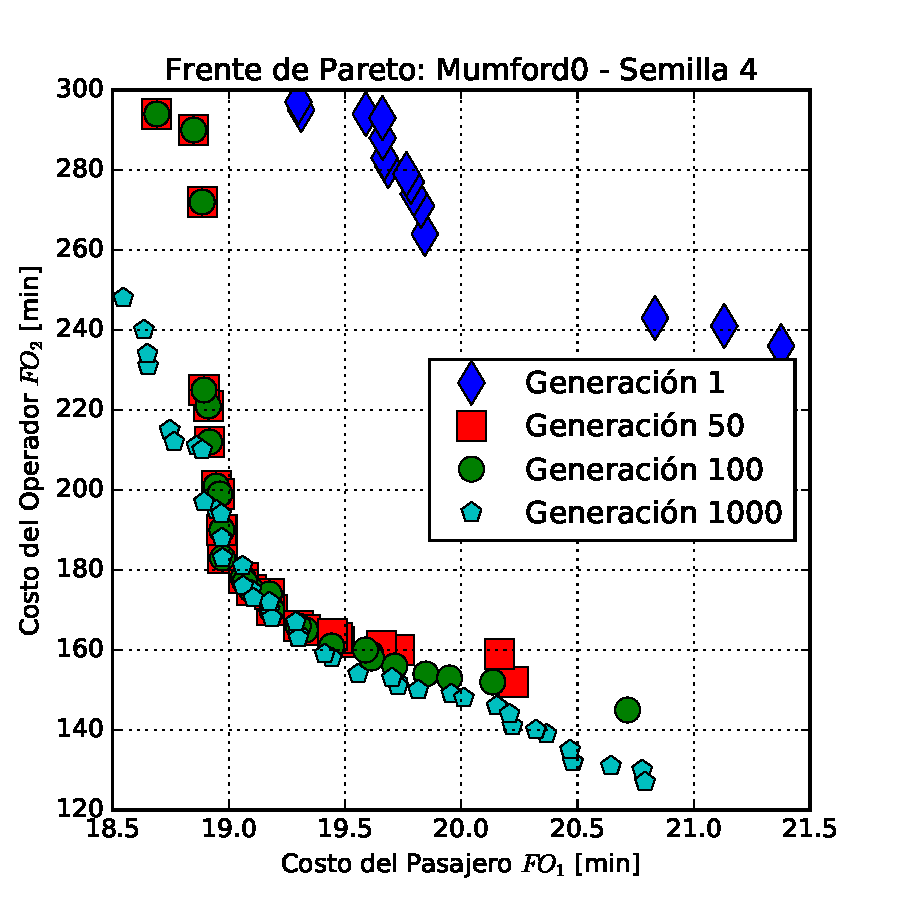
\includegraphics[width=0.79\textwidth]{img/frente_Mumford0_s4}
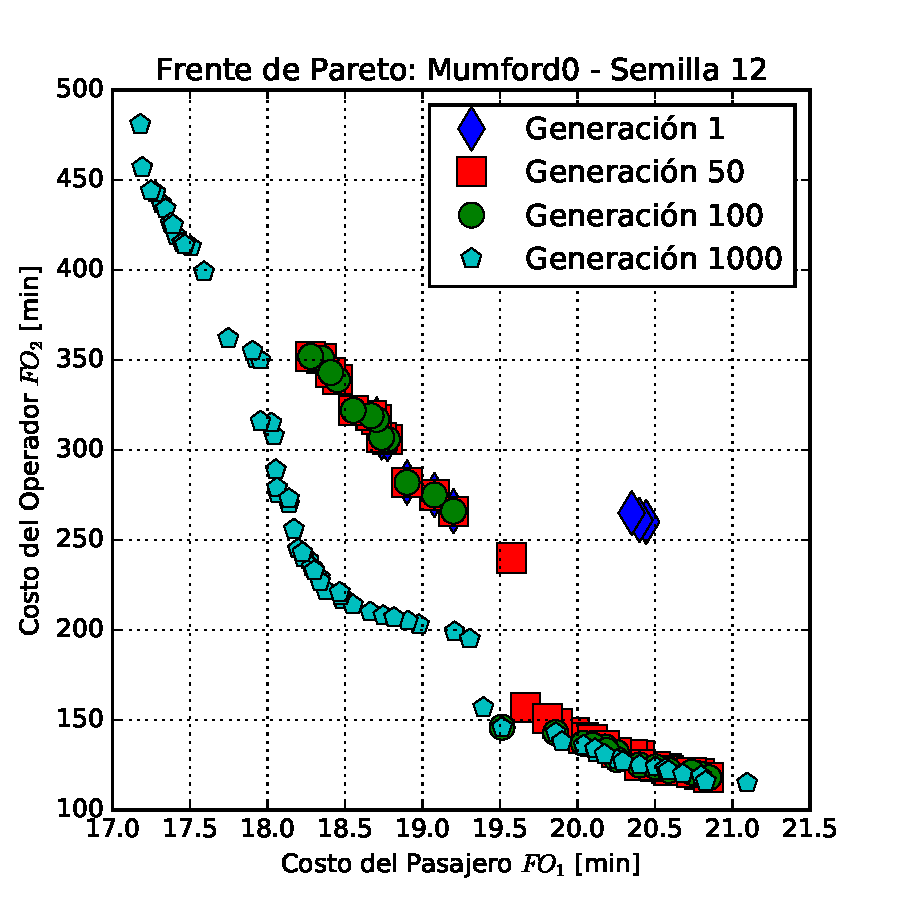
\includegraphics[width=0.79\textwidth]{img/frente_Mumford0_s12}
\caption{Frente de Pareto para Mumford0 con semillas 4 y 12.}
\label{fig:paretoMumford1}
\end{figure}

\begin{figure}[p]
\centering
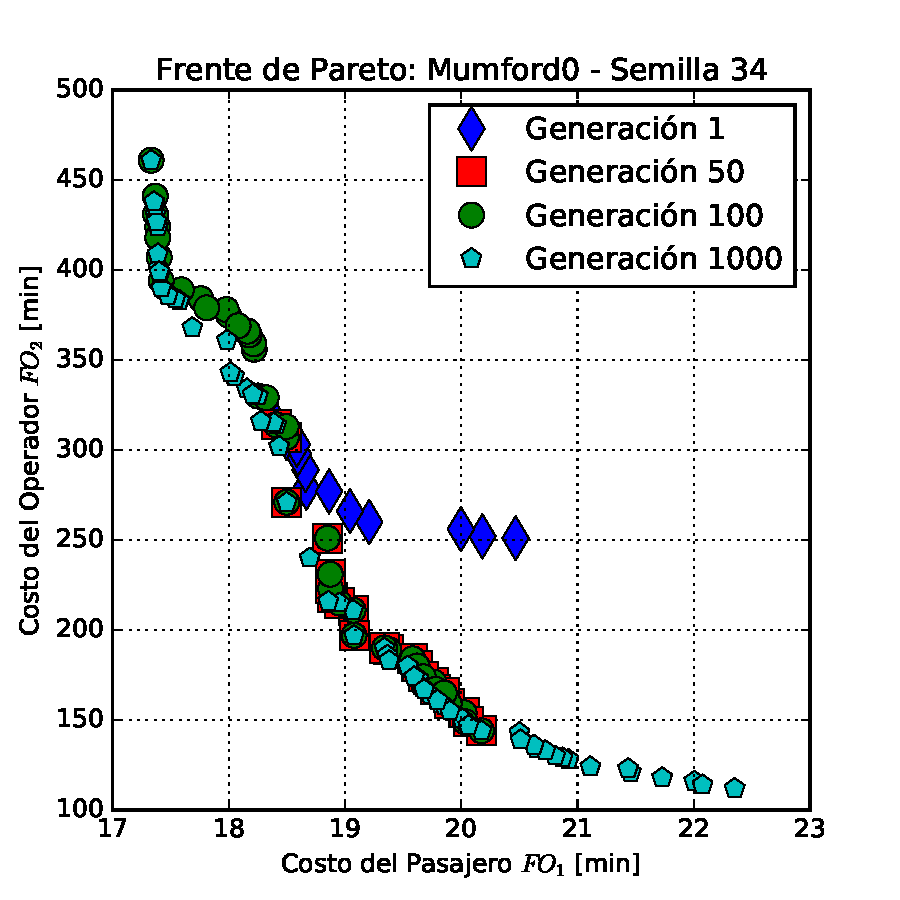
\includegraphics[width=0.79\textwidth]{img/frente_Mumford0_s34}
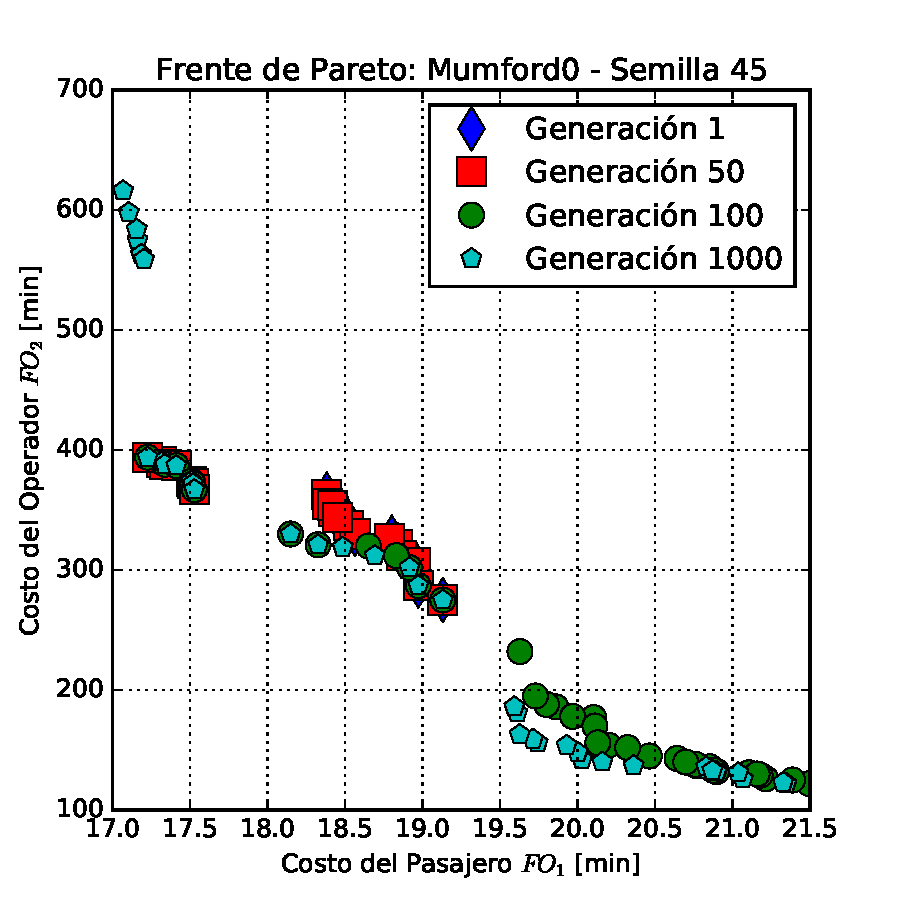
\includegraphics[width=0.79\textwidth]{img/frente_Mumford0_s45}
\caption{Frente de Pareto para Mumford0 con semillas 34 y 45.}
\label{fig:paretoMumford2}
\end{figure}

\begin{table}[!htb]
\centering
\begin{tabular}{|r|r|r|r|r|r|}
\hline
Semilla & Generación & Sol. Únicas & Sol. Totales & Hipervolumen & Tiempo [s]\\  
\hline \hline
4 & 1 & \textbf{15} & \textbf{15} & 7118.92 & \textbf{46} \\ \hline
45 & 1 & 12 & 12 & 7054.21 & 52 \\ \hline
12 & 1 & 9 & 9 & 7125.38 & 55 \\ \hline
34 & 1 & 12 & 12 & \textbf{7392.27} & 49 \\ \hline\hline
4 & 50 & 23 & 23 & 8650.36 & \textbf{1219} \\ \hline
45 & 50 & 20 & 20 & 7502.79 & 1742 \\ \hline
12 & 50 & \textbf{30} & \textbf{30} & \textbf{9185.21} & 1349 \\ \hline
34 & 50 & 22 & 22 & 8874.78 & 1276 \\ \hline\hline
4 & 100 & 26 & 33 & 8740.11 & \textbf{2280} \\ \hline
45 & 100 & 38 & 38 & \textbf{9506.56} & 3062 \\ \hline
12 & 100 & 27 & 30 & 9204.48 & 2622 \\ \hline
34 & 100 & \textbf{42} & \textbf{42} & 9285.58 & 3158 \\ \hline\hline
4 & 1000 & 42 & \textbf{103} & 9064.71 & \textbf{24308} \\ \hline
45 & 1000 & 38 & 38 & 9566.61 & 31216 \\ \hline
12 & 1000 & 64 & 85 & \textbf{9792.15} & 27600 \\ \hline
34 & 1000 & \textbf{65} & 83 & 9691.16 & 27324 \\ \hline
\end{tabular}
\caption{Cantidad de soluciones únicas/totales, hipervolumen y tiempo de cómputo en el frente de Pareto para 4 semillas de la instancia Mumford0.}
\label{tab:dataFrenteMumford0}

\vspace{0.7cm}

\end{table}

Las Figuras \ref{fig:paretoMumford1} y \ref{fig:paretoMumford2} muestran la evolución del frente de Pareto en 4 semillas distintas y la Tabla \ref{tab:dataFrenteMumford0} muestra información adicional respecto a estos frentes. Se puede apreciar que la evolución del frente para semillas presenta un comportamiento favorable, ya que se acerca a la región de mínimos en ambas funciones objetivo. Un caso notable a mencionar ocurre con la semilla 4, donde se observa un gran avance a partir del frente inicial en la primera generación hasta el frente obtenido en la generación 50. A diferencia de la instancia Mandl, en estos casos se obtiene una buena cantidad de soluciones que son mejores para operadores y para pasajeros y el algoritmo tiene ciertas dificultades para acercarse a soluciones ubicadas en la zona inferior izquierda donde está el mínimo para operadores y pasajeros simultáneamente.

Al analizar los resultados de la Tabla \ref{tab:dataFrenteMandl} se puede observar que, en general, existe una repetición de soluciones candidatas que aumenta a medida que transcurren las generaciones. En esta instancia la cantidad de soluciones únicas representan una mayor parte de las soluciones totales que en la instancia Mandl. En las cuatro semillas mostradas, las soluciones únicas representan más del 40 \% de las soluciones totales en la milésima generación. En la semilla 45 en específico, la cantidad de soluciones únicas es igual a la cantidad de soluciones totales. Nuevamente, no es posible relacionar la cantidad de soluciones con el hipervolumen obtenido para una misma semilla en una generación determinada. Además, tampoco es posible afirmar que una semilla que inicia con un buen valor de hipervolumen, seguirá siendo la mejor semilla en la generación 1000. Los tiempos registrados al finalizar una generación dan cuenta de la misma relación que en Mandl, donde semillas que tardan menos tiempo en llegar a una generación tempranamente mantendrán la tendencia y demorarán menos tiempo en terminar con las 1000 generaciones. 

La Tabla \ref{tab:mejoresfo1} muestra la mejor solución obtenida para los pasajeros en cada instancia, utilizando los valores de los parámetros sintonizados. En ninguno de los dos casos se logró llegar a la cotas inferiores dadas por $LB_{FO_1}$ según la Tabla \ref{tab:norm}, donde en el caso de Mandl la mejor solución tarda 0.47 minutos más que la cota inferior y en Mumford0 la mejor solución tarda 4.05 minutos más que la cota inferior. Las mejores soluciones para pasajeros están compuestas en su totalidad por rutas extensas.

\begin{table}[!htb]
\begin{center}
\begin{tabular}{|p{0.14\textwidth}|p{0.36\textwidth}|p{0.50\textwidth}|}
\hline
\multirow{2}{*}{Instancia} & \multicolumn{2}{c|}{Mejor solución para pasajeros (sintonización)} \\
\cline{2-3}
 & Costos & Rutas\\
\hline
\hline
Mandl & $FO_1 = 10.4778$\newline $FO_2 = 158$ \newline (semilla=4) & 9-15-6-3-2-1 \newline 3-2-5-4-6-8-10 \newline 4-2-3-6-15-7 \newline 11-10-8-6-3-2-1 \newline 9-15-7-10-11-12-4-2 \newline 11-13-14-10-7 \\
\hline
Mumford0 & $FO_1 = 17.0681$ \newline $FO_2 = 616$ \newline (semilla=45) & 8-29-17-3-16-22-7-14-1-13-9-20-18-12 \newline 24-15-2-5-4-10 \newline 27-1-26-12-15-8-3-7-6-16-11 \newline 2-5-25-8-3-30-28-16-22-11-7-6 \newline 18-1-14-7-6-22-3-16-30-28-8-5-2 \newline 27-9-13-20-23-18-1-19-14-7-3-28-17-8 \newline 7-3-11-17-16-28-8-21-15-10 \newline 7-14-19-1-26-23-18-12-4-2-5 \newline 21-8-26-1-13-9 \newline 4-2-5-8-3-7-14-19-13-23-1-20-18-12-15 \newline 30-3-22-6-16-7-14-1-20-18-29-17-28-11-8 \newline 28-11-22-6-7-17-16-3-8-25-2-4-5-15\\
\hline
\end{tabular}
\end{center}
\caption{Mejores soluciones para pasajeros por instancia.}
\label{tab:mejoresfo1}
\end{table}

Por otra parte, la Tabla \ref{tab:mejoresfo2} muestra la mejor solución para los operadores en cada instancia, utilizando los valores de parámetros sintonizados. Al comparar los valores obtenidos con las cotas inferiores de la Tabla \ref{tab:norm}, se logró llegar a la cota inferior de 63 minutos para la instancia Mandl, mientras que en Mumford0 se llegó a una solución que excede en 18 minutos a la cota inferior. Las soluciones obtenidas se caracterizan por ser rutas cortas en su mayoría. En cada caso una de las rutas del conjunto es considerablemente más extensa que el resto.

\begin{table}[!htb]
\begin{center}
\begin{tabular}{|p{0.14\textwidth}|p{0.36\textwidth}|p{0.50\textwidth}|}
\hline
\multirow{2}{*}{Instancia} & \multicolumn{2}{c|}{Mejor solución para operadores (sintonización)}\\
\cline{2-3}
 & Costos & Rutas \\
\hline
\hline
Mandl & $FO_1 = 13.0501$\newline $FO_2 = 63$ \newline (semilla=567)  & 11-13-14 \newline 9-15-7 \newline 15-8-6-3-2-4-5 \newline 2-1 \newline 7-10 \newline 12-11-10 \\
\hline
Mumford0 & $FO_1 = 22.3516$ \newline $FO_2 = 112$ \newline (semilla=34) & 15-21 \newline 5-25-15 \newline 3-30-11-7 \newline 22-11 \newline 28-17-7-6 \newline 29-26-12 \newline 19-1 \newline 16-7-14 \newline 2-4-10-24 \newline 2-5-8-29-18-19-13-20-9-27 \newline 1-23 \newline 14-1 \\
\hline
\end{tabular}
\end{center}
\caption{Mejores soluciones para operadores por instancia.}
\label{tab:mejoresfo2}
\end{table}


La Tabla \ref{tab:compmejores} condensa los resultados asociados a los mejores valores de funciones objetivo obtenidos para Mandl y Mumford0 y los compara con las cotas inferiores de cada una de estas instancias.

\begin{table}[!htb]
\begin{center}
\begin{tabular}{|l|r|r|r|r|}
\hline
Instancia & $LB_{FO_1}$ & Mejor $FO_1$ & $LB_{FO_2}$ & Mejor $FO_2$\\ \hline \hline
Mandl & 10.0058 & 10.4778 & \textbf{63} & \textbf{63}\\ \hline
Mumford0 & 13.0121 & 17.0681 & 94 & 112\\ \hline
\end{tabular}
\end{center}
\caption{Tabla resumen comparativa con mejores valores de funciones objetivo para operadores y pasajeros.}
\label{tab:compmejores}
\end{table}

Un último resultado comparativo se obtiene utilizando una población inicial de 200 y 200 generaciones, según se explica en \cite{john2014improved}. Para esto se intentó replicar tanto como sea posible el mismo experimento, considerando las diferencias existentes con el algoritmo inmune propuesto. para esto se ejecutó el algoritmo inmune con 20 semillas, manteniendo los parámetros, con excepcion de \popsize{} y \generaciones{}, en los valores obtenidos en la sintonización de parámetros. La Tabla \ref{tab:compliteratura} muestra los resultados obtenidos con el MOEA propuesto por Mumford, mejorado con una heurística mencionada en \cite{john2014improved} y denotado por MOEA-H con el algoritmo inmune propuesto, mencionado como AIA.

\begin{table}[!htb]
\begin{center}
\begin{tabular}{|l|c|r|r|r|r|}
\hline
 & & \multicolumn{2}{c|}{Mandl} & \multicolumn{2}{c|}{Mumford0} \\ \cline{3-6}
 & & MOEA-H & AIA & MOEA-H & AIA\\ \hline \hline
Mejor para & $FO_1$ & \textbf{10.25} & 10.52 & \textbf{15.40} & 17.34\\ \cline{2-6}
pasajeros & $FO_2$ &212 & 149 & 745 & 439\\ \hline
Mejor para & $FO_1$ & 13.48 & 12.97 & 32.78 & 21.41\\ \cline{2-6}
operadores & $FO_2$ & \textbf{63} & \textbf{63} & \textbf{95} & 116\\ \hline
\end{tabular}
\end{center}
\caption{Tabla comparativa con resultados obtenidos en \cite{john2014improved}.}
\label{tab:compliteratura}
\end{table}

Se puede observar que para la instancia Mandl, el algoritmo propuesto en la literatura es mejor que el algoritmo inmune considerando lo mejor para pasajeros. En la mejor solución para operadores, tanto el algoritmo MOEA-H como AIA logran llegar a la cota inferior de 63 minutos. No obstante, AIA logra mejorar el valor del costo de pasajeros en esta misma solución. En Mumford0, tanto para pasajeros, como para operadores el algoritmo de la literatura obtiene mejores resultados que el algoritmo inmune propuesto. A modo general, cuando se busca una mejor solución para pasajeros, AIA obtiene un menor costo para operadores que MOEA-H y cuando se busca la mejor solución para operadores, AIA obtiene un menor costo para pasajeros que MOEA-H.


